We can write:
\begin{align*}
	\hat{\bm{E}} &= \sum_l i\mathcal{E}_l\bm{\epsilon}_l e^{i(\bm{k}\cdot\bm{x} - \omega_l t)} \hat{a}_l + \hercon \\
	\hat{\bm{E}} &= \sum_l 2\mathcal{E}_l\bm{\epsilon}_l (\hat{q}_l \cos\bar{\phi}_l + \hat{p}\sin\bar{\phi}_l) &
	\bar{\phi}_l &= \omega_l t - \bm{k}_l \cdot\bm{x} + \frac{\pi}{2}
\end{align*}
These states also have orthogonality:
\begin{align*}
	\bra{q'}\ket{q} &= \delta(q-q') \\
	\bra{p'}\ket{p} &= 2\pi\delta(p-p')
\end{align*}
$q$ and $p$ establish a phase space for the field in our mode, where the total distance from the origin $r^2 = q^2 + p^2$ is related to the strength of the field, and the angle made from the $q$ axis is related to the phase of the field.
In classical physics we sit at a single point in phase space (that may move over time) but for a quantum system we see that we sit in a ``blob'' in phase space, because of the uncertainy relations implied by the fact that $q$ and $p$ don't commute.

We now turn our attention to determining the quadrature representaiton of Fock states:
\begin{align*}
	\bra{q}\ket{n} &= \psi_n(q)
\end{align*}
Which in the homework we have seen these are the Hermite Gaussian functions.
\begin{align*}
	\bra{q}\ket{n} &= \frac{1}{\sqrt{n!\sqrt{\pi}}} H_n(q)e^{-\frac{q^2}{2}}
\end{align*}
The vaccuum state therefore is:
\begin{align*}
	\frac{1}{\pi^\frac{1}{4}} e^{-\frac{q^2}{2}}
\end{align*}
Because the Hermite Gaussians are idempotes of the Fourier transform these will remain the same functions  (besides some scale factor) when looking at the $\hat{p}$ representations.

We can see that the expectation values of the numbers in the number states is:
\begin{align*}
	\bra{n}\hat{n}\ket{n} &= n \\
	\bra{n}\hat{n}^2\ket{n} &= n^2
\end{align*}
And so on and so forth, so the number states have no uncertainty in the numbers. Looking at the quadrature states:
\begin{align*}
	\bra{q}\hat{n}\ket{q} &= \bra{q}\left(\hat{q}^2 + \hat{p}^2  - \frac{1}{2}\right)\ket{q} \\
	\bra{q}\hat{n}\ket{q} &= q^2 +\bra{q}\hat{p}^2\ket{q} - \frac{1}{2}
\end{align*}
We now try to calculate this unknown quantity:
\begin{align*}
	\bra{q}\hat{p}^2\ket{q} &= \int \frac{dp'}{2\pi} \bra{q}\hat{p}^2\ket{p'}\bra{p'} \ket{q} \\
	\bra{q}\hat{p}^2\ket{q} &= \int \frac{dp'}{2\pi} \bra{q}p'\ ^2\ket{p'}\bra{p'} \ket{q} \\
	\bra{q}\hat{p}^2\ket{q} &= \int \frac{dp'}{2\pi} p'\ ^2
\end{align*}
Which blows up! Therefore these states have infinite photons in them, and infinite energy, so they can't physically be constructed.

We instead look at the expected values of the quadratures in Fock states:
\begin{align*}
	\bra{n}\hat{q}\ket{n} &= \bra{n} \frac{\hat{a} + \hat{a}^\dagger}{2} \ket{n} \\
	\bra{n}\hat{q}\ket{n} &= 0 \\
	\bra{n}\hat{q}^2\ket{n} &= \frac{1}{4}\bra{n}(\hat{a} + \hat{a}^\dagger)^2\ket{n} \\
	\bra{n}\hat{q}^2\ket{n} &= \frac{1}{4}\bra{n}(\hat{a}^2 + \hat{a}^\dagger\ ^2 + \hat{a}\hat{a}^\dagger + \hat{a}^\dagger\hat{a})\ket{n} \\
	\bra{n}\hat{q}^2\ket{n} &= \frac{1}{4}\bra{n}(1 + 2\hat{a}^\dagger\hat{a})\ket{n} \\
	\bra{n}\hat{q}^2\ket{n} &= \frac{1}{4}(2n+1)
\end{align*}
For $p$ we see:
\begin{align*}
	\bra{n}\hat{p}\ket{n} &= \bra{n} \frac{\hat{a} - \hat{a}^\dagger}{2i} \ket{n} \\
	\bra{n}\hat{p}\ket{n} &= 0 \\
	\bra{n}\hat{p}^2\ket{n} &= -\frac{1}{4}\bra{n}(\hat{a} - \hat{a}^\dagger)^2\ket{n} \\
	\bra{n}\hat{p}^2\ket{n} &= \frac{1}{4}\bra{n}(-\hat{a}^2 - \hat{a}^\dagger\ ^2 + \hat{a}\hat{a}^\dagger + \hat{a}^\dagger\hat{a})\ket{n} \\
	\bra{n}\hat{p}^2\ket{n} &= \frac{1}{4}\bra{n}(1 + 2\hat{a}^\dagger\hat{a})\ket{n} \\
	\bra{n}\hat{p}^2\ket{n} &= \frac{1}{4}(2n+1)
\end{align*}
Which is unsurprisingly exactly the same. So:
\begin{align*}
	\Delta q^2 &= \frac{2n +1}{4} \\
	\Delta p^2 &= \frac{2n +1}{4} \\
	\Delta p\Delta q &= \frac{2n +1}{4}
\end{align*}

\subsection{Coherent states}
Coherent states are eigenstates of $\hat{a}$ ($\hat{a}\ket{\alpha} = \alpha\ket{\alpha}$). Alternatively we could define these as displaced vaccuum states $\hat{D}(\alpha)\vac$, where:
\begin{align*}
	\hat{D}(\alpha) &= e^{\alpha\hat{a}^\dagger - \alpha^*\hat{a}}
\end{align*}
If we look at:
\begin{align*}
	\hat{a}\hat{D}(\alpha)\ket{0} &= \alpha\hat{D}(\alpha)\ket{0} \\
	[\hat{a},\hat{D}(\alpha)] &= \partder{\hat{D}(\alpha)}{\hat{a}^\dagger} \\
	[\hat{a},\hat{D}(\alpha)] &= \alpha \hat{D}(\alpha) \\
	[\hat{a},\hat{D}(\alpha)]\ket{0} &= \alpha\hat{D}(\alpha)\ket{0} \\
	\alpha\hat{D}(\alpha)\ket{0} &= \alpha\hat{D}(\alpha)\ket{0} \\
\end{align*}
In order to take our derivitive we needed the Baker-Cambell-Hausfourf relation. Assuming $A$ and $B$ don't commute but they both commute with their commutator, then:
\begin{align*}
	e^{A+B} &= e^{-\frac{[A,B]}{2}} e^A e^B
\end{align*}
So then:
\begin{align*}
	\hat{D}(\alpha) &= e^\frac{|\alpha|^2}{2} e^{\alpha\hat{a}^\dagger} e^{\alpha^*\hat{a}}
\end{align*}
This displacement operator displaces our state in phase space.

Looking at this in the Fock basis:
\begin{align*}
	\ket{\alpha} &= \sum_n c_n \ket{n} \\
	\alpha\ket{\alpha} &= \sum_n c_n \sqrt{n}\ket{n-1} \\
	\alpha\ket{\alpha} &= \sum_n c_{n+1} \sqrt{n+1}\ket{n} \\
	\alpha c_n &= c_{n+1} \sqrt{n+1} \\
	\frac{\alpha}{\sqrt{n+1}} c_n &= c_{n+1}  \\
	c_{n} &= \frac{\alpha^n}{\sqrt{n!}} c_0
\end{align*}
And then we can find $c_0$ via normalization. And we then see:
\begin{align*}
	\ket{\alpha} &= e^{-|\alpha|^2/2} \sum_n \frac{\alpha^n}{\sqrt{n!}} \ket{n}
\end{align*}
Looking at the quadrature:
\begin{align*}
	\bra{\alpha}\hat{q}\ket{\alpha} &= \frac{1}{2}\bra{\alpha}(\hat{a} + \hat{a}^\dagger)\ket{\alpha} \\ 
	\bra{\alpha}\hat{q}\ket{\alpha} &= \frac{1}{2}\bra{\alpha}(\alpha + \alpha^*)\ket{\alpha} \\ 
	\bra{\alpha}\hat{q}\ket{\alpha} &= \frac{1}{2}(\alpha + \alpha^*) \\ 
	\bra{\alpha}\hat{q}\ket{\alpha} &= \Re\alpha
\end{align*}
And similarly:
\begin{align*}
	\bra{\alpha}\hat{p}\ket{\alpha} &= \Im\alpha
\end{align*}
We can see that the square expectation values are:
\begin{align*}
	\bra{\alpha}\hat{q}^2\ket{\alpha} &= \frac{1}{4}\bra{\alpha}(\hat{a}^2 +\hat{a}^\dagger\ ^2 + 2\hat{a}^\dagger\hat{a} + 1)\ket{\alpha} \\
	\bra{\alpha}\hat{q}^2\ket{\alpha} &= \frac{1}{4}\bra{\alpha}(\alpha^2 +\alpha^*\ ^2 + 2|\alpha|^2 + 1)\ket{\alpha} \\
	\bra{\alpha}\hat{q}^2\ket{\alpha} &= \frac{1}{4}((2\Re\alpha)^2 + 1)
\end{align*}
And similarly:
\begin{align*}
	\bra{\alpha}\hat{p}^2\ket{\alpha} &= \frac{1}{4}((2\Im\alpha)^2 + 1)
\end{align*}
So then our uncertainties are:
\begin{align*}
	\Delta q^2 &= \frac{1}{4} \\
	\Delta p^2 &= \frac{1}{4} \\
	\Delta q\Delta p &= \frac{1}{4}
\end{align*}
But this is the minumum possible uncertainty! We say coherent states are ``closest'' to a classical EM field. We call the uncertainty in this state the vaccuum fluctuations of the electric field.
This vaccuum fluctuation causes many physical effects, such as the finite lifetime of excited states of an atom.

\subsection{Beam splitters}
A beam splitter splits the amplitude of the electromagnetic field. It converts between modes of the EM field. We can express the fields going through the beam splitter as:
\begin{figure*}[h]
	\centering
	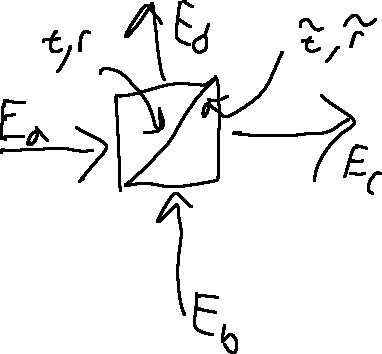
\includegraphics[width=10cm]{1-29-1.png}
	\caption*{Beamsplitter diagram}
\end{figure*}
\begin{align*}
	E_d &= rE_a + \tilde{t} E_b \\
	E_c &= tE_a + \tilde{r}E_b
\end{align*}
This is a unitary transformation so we see no loss. We can rewrite this in terms of creation/annihilation operators:
\begin{align*}
	\begin{pmatrix}
		\hat{c} \\
		\hat{d}
	\end{pmatrix} &= \begin{pmatrix}
	t & \tilde{r} \\
	r & \tilde{t}
		 \end{pmatrix}
		 \begin{pmatrix}
			 \hat{a} \\
			 \hat{b}
		 \end{pmatrix}
\end{align*}
It happens that in order to enforce unitarity we must have either:
\begin{align*}
	U &= \begin{pmatrix}
		t & r \\
		-r & t
	     \end{pmatrix} \\
	U &= \begin{pmatrix}
		t & ir \\
		ir & t
	     \end{pmatrix}
\end{align*}
We often have 50:50 beam splitters where $t=r=\frac{1}{\sqrt{2}}$ so:
\begin{align*}
	U &= \frac{1}{\sqrt{2}} \begin{pmatrix}
		1 & 1 \\
		-1 & 1
				\end{pmatrix}
\end{align*}
